%%%%%%%%%%%%%%%%%%%%%%%%%%%%%%%%%%%%%%%%%
% University of Amsterdam master thesis title page 
% LaTeX Template
%
% Version 1.2 (14/02/14) (fixed cursive mode under titlepage)
%
% This template was made for the UvA by Ludo Nieuwenhuizen
% 
% 
% Instructions for using this template:
%
% I've done my best to make this template self-explanatory. The only thing (apart from
% finishing your thesis) is that wherever you see the percentage sign after some LaTeX
% commands, you have to insert some text (except for this
% introductory part, of course)l this is also explicitly stated.
%
% This title page can be compiled as is. This is not useful for 
% including it in another document. To do this, you have two options: 
%
% 1) Copy/paste everything between \begin{document} and \end{document} 
% starting at \begin{titlepage} and paste this into another LaTeX file where you 
% want your title page.
% OR
% 2) Remove everything outside the \begin{titlepage} and \end{titlepage} and 
% move this file to the same directory as the LaTeX file you wish to add it to. 
% Then add \input{./titlepage_master_thesis.tex} to your LaTeX file where you want your
% title page.
%
% The layout is quite vulnerable for changes. If you for instance remove the logo at the
% bottom, the last line 'Department Research institute...' will get higher up the page. In this 
% case it is safer to insert a blank image or fix it in a different way.
%
% Any questions can be sent to me (L.G.Nieuwenhuizen@gmail.com)
%%%%%%%%%%%%%%%%%%%%%%%%%%%%%%%%%%%%%%%%%

\documentclass[11pt,twoside,a4paper,fleqn]{report}

\usepackage{graphicx}
\usepackage{graphics}
\usepackage[english]{babel}
\usepackage[hcentering,bindingoffset=8mm]{geometry}
\usepackage[utf8]{inputenc}
% \usepackage[en-US]{datetime2}
\usepackage{amssymb}
\usepackage{amsmath}
\usepackage{natbib}
\usepackage[colorlinks=true, allcolors=blue]{hyperref}
\usepackage{caption}
\usepackage{tocloft}
\usepackage{amsfonts}
\usepackage[section]{placeins}
\usepackage{fancyhdr}
% \usepackage{siunitx}
\usepackage{subcaption}
\usepackage{listings}
\usepackage{acro}
% \usepackage{abbriv}
\usepackage{longtable}
\usepackage{array}
\usepackage{tablefootnote}
\usepackage{epigraph}
\usepackage[capitalise]{cleveref}
\usepackage{comment}
\usepackage{float}

\graphicspath{{folder/}{../figures/}}

\pagestyle{fancy}
\fancyhead[RO]{\fancyplain{}{\nouppercase{\leftmark}}}
\renewcommand\sectionmark[1]{\markboth{\MakeUppercase{#1}}{}}
\fancyhead[LO]{}
\fancyhead[LE]{\fancyplain{}{\nouppercase{\leftmark}}}
\renewcommand\sectionmark[1]{\markboth{\MakeUppercase{#1}}{}}
\fancyhead[RE]{}
\lfoot{}
\cfoot{\fancyplain{}{\thepage}}
\rfoot{}

% \sisetup{separate-uncertainty, multi-part-units = brackets}
% \DeclareSIUnit\parsec{pc}
% \DeclareSIUnit\photons{ph}
% \def\kms{km~s$^{-1}$}

\newcolumntype{L}[1]{>{\raggedright\let\newline\\\arraybackslash\hspace{0pt}}m{#1}}

%\setlength{\headheight}{15pt}

%\parskip = \baselineskip

\captionsetup[table]{name=Table,labelfont={sc,footnotesize},textfont=footnotesize,labelsep=none}
\captionsetup[figure]{name=Fig.,labelfont={sc,small},textfont=footnotesize,labelsep=endash}
\numberwithin{equation}{chapter}
\numberwithin{figure}{chapter}

\newcommand{\vdag}{(v)^\dagger}
\newcommand\aastex{AAS\TeX}
\newcommand\latex{La\TeX}

\setlength{\parindent}{0 cm}
\pagenumbering{gobble}

\acsetup{list-style=longtable}

\begin{document}
\begin{titlepage}

\newcommand{\HRule}{\rule{\linewidth}{0.8mm}}
\center
 \vspace*{0.5cm}  % Play around with this as you want
% ------
% Heading20
% ------
\raisebox{0.05cm}[0pt][0pt]{
\includegraphics[width=2.0cm]{Thesis/logos/UvA_logo.png}}
\raisebox{0.7cm}[0pt][0pt]{\textsc{\Huge University of Amsterdam}}
\raisebox{-1.85cm}[0pt][0pt]{
\includegraphics[width=7.0cm]{Thesis/logos/VUlogo.png}}\\[2.0 cm]

\Large{\textbf{MSc Physics and Astronomy}}\\% Study discipline
\Large{Track: Astronomy \& Astrophysics}\\[0.7cm] % Master track name
\textsc{\Large \textbf{Master Thesis}}\\[0.2cm]

% -----
% Title
% -----

\HRule \\[0.3cm]

{ \huge \bfseries The evolution of TIC 470710327 hierarchical triple system with a Roche lobe filling outer star }\\[0.8cm] % title of thesis
%{\Large \bfseries Subtitle of Thesis\\Can use two lines} % subtitle of thesis

\HRule \\[0.7cm]
 
% -----
% Details
% -----

{\Large \emph by}\\[0.6cm]
{\Large \bfseries Adam Parkosidis\\ % student name
13950142}\\[0.4cm] %student ID
%\DTMlangsetup{showdayofmonth=false}
{\large  \emph{\today}}\\ % month + year in which the thesis was concluded
%\DTMlangsetup{showdayofmonth=true}
{\large  \emph{60 ECTS}}\\ % 'this many' ects that are rewarded for the thesis
{\large  \emph{Start date - End date}}\\[1.8cm] % period in which the research was carried out

% -----
% Supervisor, etc.
% -----

\begin{minipage}{0.4\textwidth}
\begin{flushleft} \large
{\large \emph{Supervisors:}}\\

\large{Dr Silvia Toonen}\\ % Supervisor's Name
\large{Dr Philipp Moesta}
\end{flushleft}
\end{minipage}
~
\begin{minipage}{0.4\textwidth}
\begin{flushright} \large
\emph{Examiners} \\
\large{Dr. Silvia Toonen} \\
\large{Dr. Oliver Porth} % Examiner's Name
\end{flushright}
\end{minipage}\\


% -----
% Logo and Department
% -----

\raisebox{-138pt}[0pt][0pt]{\includegraphics[width=5.5cm]{Thesis/logos/api_logo.pdf}}\\ % Call your institute logo "institute.jpg", or be creative.

% \raisebox{-138pt}[0pt][0pt]{\large{Anton Pannekoek Institute for Astronomy}} %name of the department or institute or company


% -----
% That was easy, right?
% -----

\vfill 

\end{titlepage}

\newpage
\chapter*{Abstract}

Mass transfer in hierarchical triple systems, and more specifically, \ac{rlof} by the outer star, is expected to be considerably different from mass transfer in an ordinary binary system. The mass cannot be simply accreted by the inner objects, but may instead form a circumbinary disk or be expelled via a slingshot effect due to the inner binary rotation. Stellar evolution, gravitational dynamics, and hydrodynamics all play important roles in the process. In the first part, we create 3D hydrodynamical models of post main-sequence stars based on detailed 1D stellar evolution models. In the second part, we use AMUSE to couple hydrodynamics with high accuracy gravitational integrators and solve these physical processes in a self-consistent  manner. Hence, we simulate the phase of mass transfer in a hierarchical triple system in which the tertiary star will overfill its Roche lobe before any of the inner stars leave the main sequence. We encounter a fairly non-conservative mass transfer, and while we quantify its impact on the inner and outer orbits, predicting the end of the mass transfer phase and the appearance of the resulting system is difficult. However, we provide some preliminary estimations of the system's accretion efficiency and the amount of angular momentum lost. Finally,
we speculate that the formation of a circumbinary disk around the inner binary probably leads to significantly more conservative mass transfer. 





\mbox{}


\newpage
\pagenumbering{roman}
\setcounter{page}{1}
{
  \hypersetup{linkcolor=black}
\tableofcontents

\begin{comment}
\newpage
\thispagestyle{empty}
\mbox{}
\newpage



\listoffigures

\newpage
\thispagestyle{empty}
\mbox{}
\newpage

\listoftables

\newpage
\thispagestyle{empty}
\mbox{}
\newpage

\mbox{}
\thispagestyle{empty}
\printacronyms[include-classes=abbrev,name=List of Abbreviations]

\end{comment}

\newpage
\thispagestyle{empty}
\mbox{}
\newpage

\pagenumbering{arabic}
\setcounter{page}{1}

}

\parskip = 2mm

\chapter{Introduction}

\epigraph{The universe must be full of voices, calling from star to star in a myriad tongues. One day we shall join that cosmic conversation}{Arthur C. Clarke}

Observations proved that field stars are not always single; many develop in pairs, and many of these binaries are members of triples or higher-order systems. Additionally, the fraction of systems with companions grows with mass (see \cref{fig:stellar_companions}), as a result massive stars are seldomly formed in isolation. In contrast, most of massive stars are created in binary or higher order multiple systems with $\sim 50\%$ of spectral type B stars be in triples \citep{sana2014southern,moe2017mind}, a percentage which reduces to $\sim 10\%$ for low-mass stars \citep{raghavan2010survey,toonen2014popcorn,moe2017mind}. In these cases, apart from the intrinsic stellar properties, the evolution depends sensitively on the interaction between the system's stellar components. Consequently, triple systems are not as uncommon as we may mistakenly believe, particularly in the concept of massive stars, the life cycle of which is still poorly understood.

Although the fundamentals of single and binary evolution have long been acknowledged \citep{postnov2014evolution,toonen2014popcorn}, the long-term evolution of stellar triples remains unknown. In the simple case, stable triple systems, which are hierarchical, namely, consist of an inner and an outer binary orbit, i.e., the tertiary (third object). The secular evolution of such systems is the modification of orbital elements over timescales substantially larger than the system's dynamical timescale. Hence, the presence of the outer star has no influence on the history of the inner binary and the evolution of the inner binary and the tertiary can be discussed independently. In other cases, a third star in orbit around a binary system can drastically influence the system's development
via dynamical interactions, which influence the orbital elements of the inner and outer orbit through changes in energy and angular momentum. Consequently, hierarchical triple star systems can become unstable via triple stellar evolution processes which are unique to systems with multiplicities of higher orders than binaries.
\begin{figure}[H]
    \centering
    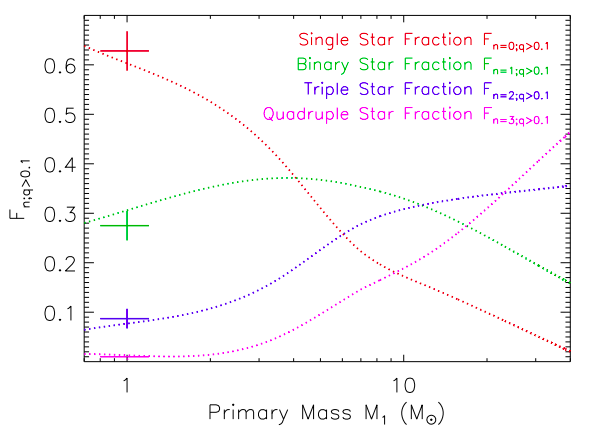
\includegraphics[width=\textwidth]{Thesis/figures/fig_moe_2017.png}
    \caption{Multiplicity fractions as a function of primary mass (dotted lines), including the single-star $F_{n=0;q> 0.1}$ (red), binary-star $F_{n=1;q> 0.1}$  (green), triple-star $F_{n=2;q> 0.1}$  (blue), and quadruple-star fraction $F_{n=3;q> 0.1}$  (magenta). Given a primary mass $M_1$, the model assumes that the multiplicity fractions follow a Poisson distribution across the interval $n = [0, 3]$ in a manner that reproduces the measured multiplicity frequency $F_{mult;q >0.1} = \Sigma_{n=1}^3 \; n F_{n;q> 0.1}$. For solar-type stars, this model matches the measured values (solid) within their uncertainties. Regardless of the uncertainties in the multiplicity fractions, $\leq 10\%$ of O-type stars are single while $\geq 55\%$ are born in triples and/or quadruples. Figure taken by \cite{moe2017mind}.}
    \label{fig:stellar_companions}
\end{figure}
The rich dynamical behavior of three-body systems can produce Lidov-Kozai cycles, in which the eccentricity of the inner orbit and the inclination between the inner and outer orbits vary periodically \citep{michaely2014secular,toonen2016evolution,mangipudi2022extreme}. As a result, tidal effects (tidal friction), gravitational-wave emission, and stellar interactions such as mass transfer, angular momentum exchange and collisions may be enhanced. In this way, evolution in triples can give rise to stellar mergers \citep{antonini2017binary,silsbee2017lidov,vigna2021massive}, namely some of most energetic events in the universe, ranging from gravitational wave sources to electromagnetic transients, e.g. luminous red novae, and also provide promising evolutionary pathways for exotic objects \citep{sana2012binary, toonen2016evolution}, e.g. blue stragglers \citep{winn2009spin}. In the past, most of our efforts in understanding the progenitors of the events were focused on modeling binary evolution disregarding the interaction of the binary with a third star. Therefore, a detailed examination of triple evolution is as necessary as it is challenging because it demands a self consistent treatment of three-body dynamics and stellar evolution.

In this thesis, I present the evolution of TIC 470710327 \citep{eisner2022planet}, a massive hierarchical triple system with a Roche lobe filling outer star. I use the Astrophysical Multipurpose Software Environment (AMUSE, \cite{portegies2018astrophysical}) to simulate the system's evolution and try to predict its future. Initially, I create stellar evolution models of the triple components until the tertiary fills its Roche lobe. I then simulate in detail the mass transfer for several orbits of the outer star using a combination of gravitational dynamics and hydrodynamics. I examine the importance of various parameters, properties and type of mass transfer, the response of the inner and outer orbital parameters, and the consequent evolution.

In the remainder of this first Chapter, I will present an overview of single massive star evolution until the end of helium burning phase with a focus on those aspects that are relevant for triple evolution. Furthermore, I will introduce concepts of binary evolution and I will argue how to extend these to the triple evolution case. After, presenting all the important concepts, I will introduce our target system, the goal and the outline of this project. 


\section{Goal \& Scientific Questions}

In this thesis, I present the evolution of TIC 470710327 \citep{eisner2022planet}, a massive hierarchical triple system with a Roche lobe filling outer star. I use the Astrophysical Multipurpose Software Environment (AMUSE, \cite{pelupessy2013astrophysical,portegies2018astrophysical}) to simulate the system's evolution and try to predict its future. Initially, I create stellar evolution models of the triple components until the tertiary fills its Roche lobe. I then simulate in detail the mass transfer for several orbits of the outer star using a combination of gravitational dynamics and hydrodynamics. 

There are two main scientific questions that I try to tackle:

\begin{itemize}
    \item How the mass transfer affects the orbital parameters of the two orbits?
    \item How the accretion of the binary affects the orbital parameters of the two orbits?
\end{itemize}

I examine the importance of various parameters, properties and type of mass transfer, the response of the inner and outer orbital parameters, and the consequent evolution.





\section{Thesis Outline}
This thesis is structured as follows: 

In the second chapter, I present an overview of single massive star evolution until the end of helium burning phase with a focus on those aspects that are relevant for triple evolution. Furthermore, I discuss concepts of binary evolution and I argue how to extend these to the triple evolution case. In the remainder of this chapter, I provide information about the scientific codes utilized in my simulations. In chapter three, I introduce my target system. In the fourth chapter, I display the setup of my simulations, the underlying assumptions of my models, and their physical justification.



%\subsection{AMUSE}

\section{Hierarchical Triple Star Systems}

\section{Goal and Outline of Thesis}

%\subsection{AMUSE}

\subsection{Thesis Outline}
This thesis is structured as follows: i








\chapter{TIC 470710327}

\epigraph{The universe must be full of voices, calling from star to star in a myriad tongues. One day we shall join that cosmic conversation}{Arthur C. Clarke}

\chapter{Simulations}

%\epigraph{The stars are not distant objects to be admired from afar. They are our partners in exploration and discovery, and we must learn to live and work with them if we are to achieve our goals.}{Arthur C. Clarke}

The evolution of outer Roche lobe overflow (RLOF) triple-star systems is influenced by various physical processes, including stellar evolution, gravitational dynamics, and hydrodynamics. I utilize the Astrophysical Multi-purpose Software Environment (AMUSE, \cite{portegies2018astrophysical}), a comprehensive computational tool, to accurately simulate and solve for these physical processes in a self-consistent manner. To model the evolution of the system star prior to outer stars's RLOF, I employed a stellar evolution code (MESA, \cite{paxton2010modules,paxton2013modules,paxton2015modules,paxton2019modules}). Once the outer star reached the stage where it approximately filled its Roche lobe, I pause the stellar evolution simulation and converted the one-dimensional stellar structure into a three-dimensional hydrodynamical model. This hydrodynamical model of the outer star is then relaxed and placed in orbit around the binary star. Subsequently, I monitor the intricate hydrodynamics of the mass transfer from the Roche lobe-filling outer star to the inner binary for multiple orbits, while simultaneously keeping track of the gravitational dynamics of the three stars and the hydrodynamics of the gas from the outer star. A schematic representation of the entire process is provided in 

\section{Stellar Evolution}

MESA (Modules for Experiments in Stellar Astrophysics, \cite{paxton2010modules,paxton2013modules,paxton2015modules,paxton2019modules}) is an open-source 1D stellar evolution code used to model the evolution of stars from their birth to their death. It is a Fortran code that combines many numerical and physics modules for simulations of a wide range of stellar evolution scenarios ranging from very low mass to massive stars, including advanced evolutionary phases. Key modules within MESA include the equation of state module, the nuclear reaction network module, and the hydrodynamic module. MESA also includes modules for convective and radiative energy transport, as well as modules for mass loss, rotation, and magnetic fields. 

The code's basic principle is that it solves the fully coupled structure and composition equations simultaneously. Thus, allows me to track the independent evolution of the triple system components and obtain estimations of their properties at the moment of RLOF. In addition to fundamental parameters such as mass, radius, etc., MESA enables the access to the internal structure and detailed properties of the individual components. This information is essential for the conversion of one-dimensional stellar models into three-dimensional hydrodynamical realizations, providing a more comprehensive understanding of the physical processes involved in RLOF and the resulting mass transfer in these systems.

The stellar evolution calculations in this work are performed using the normal AMUSE parameters for MESA version 2208, with solar metallicity as the input. By the time the outer star approaches the radius of its Roche lobe, it has lost some mass and its radius is much bigger than when it was born. Table includes the important parameters of the system at the moment of RLOF. Figure 3 depicts the radial density profile of the outer component of the star at the moment of RLOF (green drawn line)





%\chapter{Hierarchical Triple Star Systems}



\newpage

\bibliographystyle{plainnat}
\bibliography{refs}

%## IMPORTANT#############################################
\acuseall
%## IMPORTANT#############################################

\end{document}